\documentclass[a4paper,11pt,openright,numbers=noenddot]{scrreprt}

\usepackage[utf8]{inputenc} % Einstellung der Eingabekodierung
\usepackage[ngerman]{babel} % Deutsche Trennmuster
\usepackage{newpxtext} % Schriftart Palatino
\usepackage{newpxmath} % passende Mathe-Schrift
\usepackage[T1]{fontenc} % Einstellung Schriftkodierung
\usepackage{amsmath} % Mathematik-Erweiterungen
\usepackage{microtype} % Verbesserte Mikrotypographie
\usepackage{csquotes} % Kontextabhängige Anführungszeichen
\usepackage{calc} % Berechnung von TeX-Maßen
\usepackage[%
  inner=25mm,%
  outer=35mm,%
  top=25mm,%
  bottom=30mm,%
  includeheadfoot,%
  headheight=14pt,%
  marginparwidth=25mm%
]{geometry} % Anpassung Satzspiegel
\usepackage{array} % Tabellen-Erweiterung
\usepackage{graphicx} % Einbindung von Grafiken
\usepackage{float} % Anpassung von Gleitumgebungen
\usepackage{acro} % Abkürzungen
\acsetup{make-links = true}
\usepackage{listings} % Codeblöcke
\usepackage{pgfplots} % Plots
\pgfplotsset{compat=1.18}
\usepackage{pgfplotstable} % CSV für Plots importieren
\usepgfplotslibrary{statistics} % Boxplots
\usepackage{csvsimple} % CSV für Tabellen importieren
\usepackage{booktabs} % Tabellenlinien
\usepackage{pdfpages} % Einbindung von externen PDFs
\usepackage{letltxmacro} % redefining commands with optional arguments
\usepackage{xcolor} % for colorlet command
\usepackage{svg} % includesvg
\usepackage{subcaption} % subfigures
\usepackage{tikz}
\usetikzlibrary{shapes, calc, positioning}
\usepackage{environ} % scale tikz picture to width
\usepackage{fixltx2e} % textsubscript
\usepackage[titletoc]{appendix}

\usepackage[style=apa,backend=biber,natbib,doi=false]{biblatex}

% auf Einbindungsreihenfolge achten
\usepackage[hidelinks]{hyperref}


% können nach Fertigstellung gelöscht werden
% \usepackage{todonotes} % TODO-Anmerkungen
% \usepackage{marginnote}
% \let\marginpar\marginnote
% \usepackage{lipsum} % Blindtexte
% \usepackage{blindtext} % Blindtexte
% \usepackage{layout} % Darstellung des Satzspiegels

\floatplacement{figure}{htb}
\floatplacement{table}{htb}
   % Anpassungen für Gleitumgebungen
% Umgebung für das Deckblatt
\newenvironment{tuctitlepage}
{
  \cleardoublepage
  \titlepage
  \center
}
{
  \endcenter
  \endtitlepage
}


% Professur, Institut, ...
\newenvironment{tuctitleorgunit}{\center}{\endcenter}


% Logo
\newcommand{\tuctitlelogoname}{tuc/tuc_green_margin}

\newcommand{\tuctitlelogo}[1][0.6\linewidth]
{%
  \begin{center}%
    \includegraphics[width=#1]{\tuctitlelogoname}%
  \end{center}%
}


% Block mit kleiner Überschrift.
\newenvironment{tuctitleblock}[2][\medskipamount]
{\center\vspace*{#1}{#2\par}\vspace*{#1}}
{\par\endcenter}


% Art der Arbeit
\newcommand{\tuctitlethesistype}[1]
{\begin{center}{\huge\bfseries#1}\par\end{center}}


% Angestrebter Abschluss
\newcommand{\tuctitledegreephrase}{zur Erlangung des akademischen Grades}
\newcommand{\tuctitledegreeline}[1]
{{\LARGE #1}\par}
\newcommand{\tuctitledegree}[2][\medskipamount]
{\begin{tuctitleblock}[#1]{\tuctitledegreephrase}%
    \tuctitledegreeline{#2}%
  \end{tuctitleblock}}


% Autor
\newcommand{\tuctitleauthorphrase}{vorgelegt von}
\newcommand{\tuctitleauthorline}[1]
{{\Large #1}\par}
\newcommand{\tuctitleauthor}[2][\medskipamount]
{\begin{tuctitleblock}[#1]{\tuctitleauthorphrase}%
    \tuctitleauthorline{#2}%
  \end{tuctitleblock}}


% Lehrveranstaltung
\newcommand{\tuctitlecoursephrase}{zur Lehrveranstaltung}
\newcommand{\tuctitlecourseline}[1]
{{\LARGE #1}\par}
\newcommand{\tuctitlecourse}[2][\medskipamount]
{\begin{tuctitleblock}[#1]{\tuctitlecoursephrase}%
    \tuctitlecourseline{#2}%
  \end{tuctitleblock}}


% Semester
\newcommand{\tuctitletermphrase}{im}
\newcommand{\tuctitletermline}[1]
{{\Large #1}\par}
\newcommand{\tuctitleterm}[2][\medskipamount]
{\begin{tuctitleblock}[#1]{\tuctitletermphrase}%
    \tuctitletermline{#2}%
  \end{tuctitleblock}}


% Thema der Arbeit
\newenvironment{tuctitletopic}
{\center\LARGE\medskip\begingroup}
{\par\endgroup\medskip\endcenter}


%
% Deckblatttabellen ohne Einzug
%
% #1 -> Formatierung der linken Spalte
% #2 -> Anzahl rechter Spalten
%
\newenvironment{tuctitletable}[2][]
{\center\tabular{>{#1}r*{#2}{l}}}
{\endtabular\endcenter}


%
% Deckblatttabellen mit Einzug
%
% #1 -> Formatierung der linken Spalte
% #2 -> Anzahl rechter Spalten
% #3 -> Breite der linken Spalte
%
\newenvironment{tuctitletableindent}[3][]
{\flushleft\tabular{@{}>{\raggedleft#1}p{#3-\tabcolsep}*{#2}{l}}}%
{\endtabular\endflushleft}


% Datum, Ort
\newcommand{\tuctitleplacedate}[1]
{\center\medskip#1\par\endcenter}
 % Formatvorlage für das Deckblatt
\newenvironment{tucsimplesection}[2][\bigskipamount]
{
  \par\centerline{\textbf{\Large #2}}\par
  \vspace*{#1}
}
{}
 % Einfache Überschriften für Aufgabenstellung usw.
\newenvironment{tucerklaerung}[1][Selbstständigkeitserklärung]
{
  \pagestyle{empty}
  \thispagestyle{empty}
  \newcommand{\tucsignature}[2][5cm]%
  {
    \par
    \begin{flushright}
      \begin{minipage}{##1}
        \footnotesize
        \vbox{\hbox to \hsize{\rule{0pt}{7ex}\dotfill}\hbox{\hspace{1em}##2}}
      \end{minipage}
    \end{flushright}
  }
  \tucsimplesection{#1}
}
{
  \endtucsimplesection
}
 % Formatvorlage für die Selbstständigkeitserklärung
% https://tex.stackexchange.com/a/302313
\makeatletter
\newcommand{\newstarcommand}[1]{%
  \DeclareRobustCommand#1{%
    \@ifstar{\csname s\string#1\endcsname}{\csname n\string#1\endcsname}%
  }%
  \edef\meta@def@name{\string#1}%
  \meta@def
}
\newcommand\meta@def[3][0]{%
  \expandafter\newcommand\csname n\meta@def@name\endcsname[#1]{#2}%
  \expandafter\newcommand\csname s\meta@def@name\endcsname[#1]{#3}%
}
\makeatother

% todo footnotes
% \newcounter{todocounter}
% \setcounter{todocounter}{100}
% \newcommand{\todo}[1]{\refstepcounter{todocounter}\textcolor{red}{\footnote[\thetodocounter]{\textcolor{gray}{TODO: #1}}}}

% inline box notes
\newcommand{\boxnote}[1]{%
  \bigbreak
  \begin{center}
    \noindent\fbox{\parbox{0.85\textwidth}{#1}}
  \end{center}
  \bigbreak
}

% ignore rows in pgfplotstableread?
\pgfplotstableset{%
  cignore row/.style={
    row predicate/.append code={
      \ifnum#1=\pgfplotstablerow\relax
        \pgfplotstableuserowfalse
      \fi
    }
  },
}

% custom label
\makeatletter
\newcommand{\clabel}[2]{%
   \protected@write \@auxout {}{\string \newlabel {#1}{{#2}{\thepage}{#2}{#1}{}} }%
   \hypertarget{#1}{#2}%
}
\makeatother

% paragraph label
\newcommand{\plabel}[1]{\phantomsection\label{#1}}

% pskip
\newcommand{\pskip}{\vspace{\baselineskip}\noindent}
 % util commands
\defbibfilter{articles}{
  type=article or
  type=inproceedings or
  type=report
}

\defbibfilter{books}{
  type=book or
  type=inbook or
  type=incollection
}

\defbibfilter{software}{
  type=software
}

\defbibfilter{other}{
  not (
    type=article or
    type=inproceedings or
    type=report or
    type=book or
    type=inbook or
    type=incollection or
    type=software
  )
}

\DefineBibliographyStrings{ngerman}{
  nodate = {{}o\adddot \space D\adddot},
  mathesis = {Masterarbeit}
}

\makeatletter
% cite the alias like this: OGC (2016) or Open Geospatial Consortium (OGC) (2016)
\DeclareCiteCommand{\textcitealias}
{\usebibmacro{prenote}}
{\usebibmacro{citeindex}%
  \printtext[bibhyperref]{\@citealias{\thefield{entrykey}} (\citeyear{\thefield{entrykey}})}}
{\multicitedelim}
{\usebibmacro{postnote}}

% cite the alias like this: (OGC, 2016) or (Open Geospatial Consortium (OGC), (2016))
\DeclareCiteCommand{\parencitealias}[\mkbibparens]
{\usebibmacro{prenote}}
{\usebibmacro{citeindex}%
  \printtext[bibhyperref]{\@citealias{\thefield{entrykey}}, \citeyear{\thefield{entrykey}}}}
{\multicitedelim}
{\usebibmacro{postnote}}

% cite the alias with a forced short form like this: OGC (2016)
\DeclareCiteCommand{\textcitealiass}
{\usebibmacro{prenote}}
{\usebibmacro{citeindex}%
  \printtext[bibhyperref]{\@citealias{\thefield{entrykey}S} (\citeyear{\thefield{entrykey}})}}
{\multicitedelim}
{\usebibmacro{postnote}}

% cite the alias with a forced short form like this: (OGC, 2016)
\DeclareCiteCommand{\parencitealiass}[\mkbibparens]
{\usebibmacro{prenote}}
{\usebibmacro{citeindex}%
  \printtext[bibhyperref]{\@citealias{\thefield{entrykey}S}, \citeyear{\thefield{entrykey}}}}
{\multicitedelim}
{\usebibmacro{postnote}}
\makeatother

\defcitealias{ogcOGC}{\ac{OGC}}
\defcitealias{ogcCatalogue2016}{\ac{OGC}}
\defcitealias{ogcFiltering}{\ac{OGC}}
\defcitealias{ogcFilteringS}{\acs*{OGC}}
\defcitealias{ogcOGCAPI12022}{\ac{OGC}}
\defcitealias{ogcOGCAPI22022}{\ac{OGC}}
\defcitealias{ogcOGCAPI4}{\ac{OGC}}
\defcitealias{ISO924111}{ISO/TC 159 Ergonomics SC 4}
\defcitealias{unisd2021}{UNIS-D}
\defcitealias{bootstrapIcons}{Bootstrap Icons}
\defcitealias{scratchfoundationScratch}{Scratch}
\defcitealias{monigSnap}{\textit{Snap!}}
 % bib utils
\renewcommand{\lstlistingname}{Quelltext}
\renewcommand{\lstlistlistingname}{Quelltextverzeichnis}

\makeatletter
\let\orig@lstnumber=\thelstnumber

\newcommand\lstsetnumber[1]{\gdef\thelstnumber{#1}}
\newcommand\lstresetnumber{\global\let\thelstnumber=\orig@lstnumber}
\makeatother

\lstset{numbers=left, aboveskip=1em, captionpos=b}

\colorlet{punct}{red!60!black}
\definecolor{background}{HTML}{EEEEEE}
\definecolor{delim}{RGB}{20,105,176}
\colorlet{numb}{magenta!60!black}

\lstdefinelanguage{json}{
  basicstyle=\normalfont\ttfamily,
  numbers=left,
  numberstyle=\scriptsize,
  stepnumber=1,
  numbersep=8pt,
  showstringspaces=false,
  breaklines=true,
  frame=lines,
  backgroundcolor=\color{background},
  literate=
   *{:}{{{\color{punct}{:}}}}{1}
    {,}{{{\color{punct}{,}}}}{1}
    {\{}{{{\color{delim}{\{}}}}{1}
    {\}}{{{\color{delim}{\}}}}}{1}
    {[}{{{\color{delim}{[}}}}{1}
    {]}{{{\color{delim}{]}}}}{1},
}

\lstdefinelanguage{bnf}{
  basicstyle=\normalfont\ttfamily,
  numbers=left,
  numberstyle=\scriptsize,
  stepnumber=1,
  numbersep=8pt,
  showstringspaces=false,
  breaklines=true,
  frame=lines,
  backgroundcolor=\color{background},
  literate=
   *{=}{{{\color{punct}{=}}}}{1}
    {|}{{{\color{punct}{|}}}}{1}
    {;}{{{\color{punct}{;}}}}{1}
    {\{}{{{\color{delim}{\{}}}}{1}
    {\}}{{{\color{delim}{\}}}}}{1}
    {[}{{{\color{delim}{[}}}}{1}
    {]}{{{\color{delim}{]}}}}{1},
}

\newcommand\YAMLcolonstyle{\color{punct}\mdseries}
\newcommand\YAMLkeystyle{\color{black}\bfseries}
\newcommand\YAMLvaluestyle{\color{delim}\mdseries}

\lstdefinelanguage{yaml}{
  keywords={true,false,null,y,n},
  keywordstyle=\color{darkgray}\bfseries,
  basicstyle=\YAMLkeystyle,                                 % assuming a key comes first
  sensitive=false,
  comment=[l]{\#},
  morecomment=[s]{/*}{*/},
  commentstyle=\color{purple}\ttfamily,
  stringstyle=\YAMLvaluestyle\ttfamily,
  moredelim=[l][\color{orange}]{\&},
  moredelim=[l][\color{magenta}]{*},
  moredelim=**[il][\YAMLcolonstyle{:}\YAMLvaluestyle]{:},   % switch to value style at :
  morestring=[b]',
  morestring=[b]",
  frame=lines,
  backgroundcolor=\color{background},
  literate =    {---}{{\ProcessThreeDashes}}3
                {>}{{\textcolor{red}\textgreater}}1     
                {|}{{\textcolor{red}\textbar}}1 
                {\ -\ }{{\mdseries\ -\ }}3,
}

\lstdefinelanguage{simplexservice}{
  breaklines=true,
  frame=lines,
  backgroundcolor=\color{background},
  numbers=none,
  basicstyle=\footnotesize\ttfamily,
  keywordstyle=\color{s4d-blue},
  keywords={},
  otherkeywords={/scenarios,/\{scenarioId\}}
}

\makeatletter
% switch to key style at EOL
\lst@AddToHook{EveryLine}{\ifx\lst@language\language@yaml\YAMLkeystyle\fi}
\makeatother

\newcommand\ProcessThreeDashes{\llap{\color{cyan}\mdseries-{-}-}}
 % listings setup
\definecolor{s4d-blue}{HTML}{055DA9}

\definecolor{plot1}{HTML}{8DC144}
\colorlet{plot2}{s4d-blue}
\definecolor{plot3}{HTML}{84689B}
\definecolor{plot4}{HTML}{CF461C}
 % colors

\DeclareAcronym{2FA}{short=2FA,long=Zwei-Faktor-Authentifizierung}
\DeclareAcronym{SMS}{short=SMS,long=Short Message Service}
\DeclareAcronym{OTP}{short=OTP,long=One Time Password}
\DeclareAcronym{TOTP}{short=TOTP,long=Time-based One Time Password}
\DeclareAcronym{MIM}{short=MIM,long=Man-In-the-Middle}
\DeclareAcronym{SS7}{short=SS7,long=Signaling System 7}
 % acronyms
\newcommand{\organization}{
    Technische Universität Chemnitz \\
    Fakultät Informatik \\
    Professur Medieninformatik \\
}
\newcommand{\type}{Hauptseminar}
\newcommand{\theauthor}{Joshua Jeschek}
\newcommand{\thetitle}{Zwei-Faktor-Authentifizierung}
\newcommand{\thesubtitle}{Benutzerfreundlichkeit verschiedener Zwei-Faktor-Authentifizierungsmethoden}
\newcommand{\pruefer}{Dr. Thomas Wilhelm-Stein}
\newcommand{\place}{München}
\date{30. September 2024}

\author{\theauthor}
\title{\thetitle}
\subtitle{\thesubtitle}
 % acronyms

\hypersetup{
  pdftitle=\thetitle,
  pdfsubject=\thesubtitle,
  pdfauthor=\theauthor,
  colorlinks=false,
}

\addbibresource{bibliography.bib}

\MakeOuterQuote{"} % könnte zu Problemen führen

% \raggedbottom

\begin{document}
\pagenumbering{gobble}
\makeatletter
\begin{tuctitlepage}
  \begin{tuctitleorgunit}
    \organization
  \end{tuctitleorgunit}

  \tuctitlelogo

  \tuctitlethesistype{\type}
  \bigskip
  \tuctitleauthor{\@author}

  \vspace*{0pt plus 2fill}
  \begin{tuctitletopic}
    \@title \\
    \large{\@subtitle}
  \end{tuctitletopic}
  \vspace*{0pt plus 2fill}

  \begin{tuctitletable}[\bfseries]{1}
    Prüfer:  & \pruefer \\
  \end{tuctitletable}

  \vspace*{0pt plus 1fill}

  \tuctitleplacedate{\place, \@date}
\end{tuctitlepage}
\makeatother


\cleardoublepage
\pagenumbering{roman}
\currentpdfbookmark{Inhaltsverzeichnis}{toc}
\tableofcontents

\cleardoublepage
\begingroup
% \let\clearpage\relax
% \let\cleardoublepage\relax
\phantomsection
\addcontentsline{toc}{chapter}{\listfigurename}
\listoffigures

% \cleardoublepage
% \phantomsection
% \addcontentsline{toc}{chapter}{\lstlistlistingname}
% \lstlistoflistings
%
% \cleardoublepage
% \phantomsection
% \addcontentsline{toc}{chapter}{\listtablename}
% \listoftables
\endgroup

\cleardoublepage
\phantomsection
\addcontentsline{toc}{chapter}{Abkürzungen}
\printacronyms


\cleardoublepage
\pagenumbering{arabic}

\newcommand{\gfn}{\footnote{In dieser Arbeit wird das generische Femininum genutzt. Die in dieser Arbeit verwendeten Personenbezeichnungen beziehen sich - sofern nicht anders kenntlich gemacht - auf alle Geschlechter.}}

\chapter{Einleitung}

Passwortlecks sind ein immer wiederkehrendes Thema in den Medien. Ob durch Angriffe auf große Unternehmen \parencite{mccandlessWorldsBiggest2024}, oder zunehmend raffinierte Phishing-Attacken \parencite{colnagoItsNot2018}, die Veröffentlichung von E-Mail-Adressen und Passwörtern stellt ein erhebliches Risiko für Nutzerinnen\gfn dar. Schlechte Passwortgewohnheiten, wie die Wiederverwendung von Passwörtern oder die Nutzung leicht zu erratender Passwörter, verstärken dieses Risiko zusätzlich \parencite{colnagoItsNot2018}.

\ac{2FA} bietet jedoch einen wirksamen Schutz gegen Cyberangriffe. Durch die Verwendung eines zweiten, individuellen Sicherheitsfaktors können selbst Accounts mit schwachen oder mehrfach genutzten Passwörtern im Falle eines Datenlecks besser geschützt werden.

Trotz der zunehmenden Medienpräsenz von Datenlecks sind die Nutzungsraten von 2FA weiterhin gering \parencite{petsasTwofactorAuthentication2015, ackermanImpedimentsAdoption2020}.  Diese Diskrepanz wirft die Frage auf, warum viele Nutzerinnen \ac{2FA} nicht anwenden und wie mehr Menschen dazu bewegt werden können, diese Sicherheitsmaßnahme zu nutzen.


Die vorliegende Arbeit untersucht zunächst verschiedene \ac{2FA}-Methoden:, darunter \aclp{OTP}, \aclp{TOTP}, vor-generierte Codes, Push-Benachrichtigungen und \ac{U2F} Security Keys. Dabei werden sowohl Sicherheitsaspekte als auch die Benutzerfreundlichkeit der einzelnen Methoden beleuchtet. In Kapitel \ref{sec:adoption} wird analysiert, welche Hindernisse die Nutzung von \ac{2FA} erschweren und welche Maßnahmen zur Erhöhung der Nutzungsrate beitragen können.

\chapter{Zwei-Faktor-Authentifizierungsmethoden}
Die \ac{2FA} ist ein Sicherheitsverfahren, welches zwei unterschiedliche Komponenten zur Verifizierung der Identität von Nutzerinnen erfordert \parencite{decristofaroComparativeUsability2014}. Verschiedene Publikationen definieren dazu drei Kategorien \parencite{decristofaroComparativeUsability2014, yuEfficientGeneric2014, singhMultifactorAuthentication2017}:
\begin{itemize}
  \item \textbf{Wissen}: Etwas, was die Benutzerin weiß (z.B. Passwort, PIN)
  \item \textbf{Besitz}: Etwas, was die Benutzerin besitzt (z.B. Smartphone, Physisches Token)
  \item \textbf{Inhärenz}: Etwas, was die Benutzerin ist (z.B. Fingerabdruck, Gesichtserkennung)
\end{itemize}
Sobald Elemente aus verschiedenen Kategorien genutzt werden, handelt es sich um Multi-Faktor-Authentifizierung. Am meisten verbreitet ist \ac{2FA}, wobei Faktoren aus zwei der Kategorien abgefragt werden \parencite{decristofaroComparativeUsability2014}. Am Häufigsten wird \ac{2FA} mit einen Passwort und einem weiteren Faktor umgesetzt \parencite{decristofaroComparativeUsability2014}.

\pskip
\ac{2FA} stellt eine Verbesserung der Sicherheit gegenüber traditionellen Methoden, die nur einen Faktor verwenden (z.B. Passwörter), da es schwieriger ist, beide Faktoren zu kompromittieren \parencite{dasguptaMultiFactorAuthentication2017}.

Des Weiteren werden gängige Angriffsmethoden wie Phishing oder Keylogging erschwert. Angreiferinnen können selbst wenn sie das Passwort wissen, nicht auf die Konten der Benutzerinnen zugreifen \parencite{dasguptaMultiFactorAuthentication2017}. Auch wenn Passwörter im Rahmen eines Daten-Leaks an die Öffentlichkeit geraten, ermöglicht dies keinen sofortigen Zugriff und gibt den Betroffenen Zeit, ihr Passwort anzupassen.

\pskip
In vielen Bereichen, wie beispielsweise dem Online-Banking und Regierungsbehörden, wird \ac{2FA} eingesetzt und ist Pflicht. Dennoch ist die Entwicklung von \ac{2FA}-Methoden noch nicht abgeschlossen und birgt einige Herausforderungen.

Einerseits kann die Einführung eines zusätzlichen Authentifizierungsschrittes zu Lasten der Benutzerinnenerfahrung gehen \parencite{decristofaroComparativeUsability2014}. Andererseits werden durch zusätzliche Faktoren auch zusätzliche Implementierungskosten hervorgerufen, sei dies durch Hardware-Kosten (z.B. für Security-Tokens), technische Implementierung, oder Support \parencite{alsaleemMultiFactorAuthentication2021}.

\pskip
Im folgenden werden fünf gängige \ac{2FA}-Methoden vorgestellt. Dabei wird sowohl auf deren Funktionsweise, als auch auf Usability-Probleme und Sicherheitserwägungen eingegangen.

\section{SMS}
Sim Swapping
SS7 Attacks
\section{TOTP}
\section{Vor-Generierte Codes}
\section{Push Benachrichtigungen}
\section{U2F Security-Tokens}

% \chapter{Sicherheit der Zwei-Faktor-Authentifizierungsmethoden}

\chapter{Verbreitung von \acl{2FA}}
\label{sec:adoption}

Die Nutzungsraten von \ac{2FA} sind weiterhin gering. Laut \textcite{petsasTwofactorAuthentication2015} wenden nur 6,4\% der Nutzerinnen die Zwei-Schritt-Verifizierung von Google an, während diese Rate bei anderen Anbietern nur 2-5\% betrage. Im professionellen Bereich wurden hingegen sogar 17\% festgestellt \parencite{ackermanImpedimentsAdoption2020}. Abbildung \ref{fig:motivation} zeigt jedoch, dass in professionellen Kontexten \ac{2FA} oft nicht aus eigenem Antrieb, sondern aus Pflicht genutzt werden \parencite{decristofaroComparativeUsability2014}. Da im Privaten eine \ac{2FA}-Pflicht schwieriger durchzusetzen ist, insbesondere ohne die Nutzerinnen zu vergraulen, gilt es herauszufinden, was sie davon abhält und wie sie zur Nutzung von \ac{2FA} gebracht werden können.

\begin{figure}
  \begin{center}
    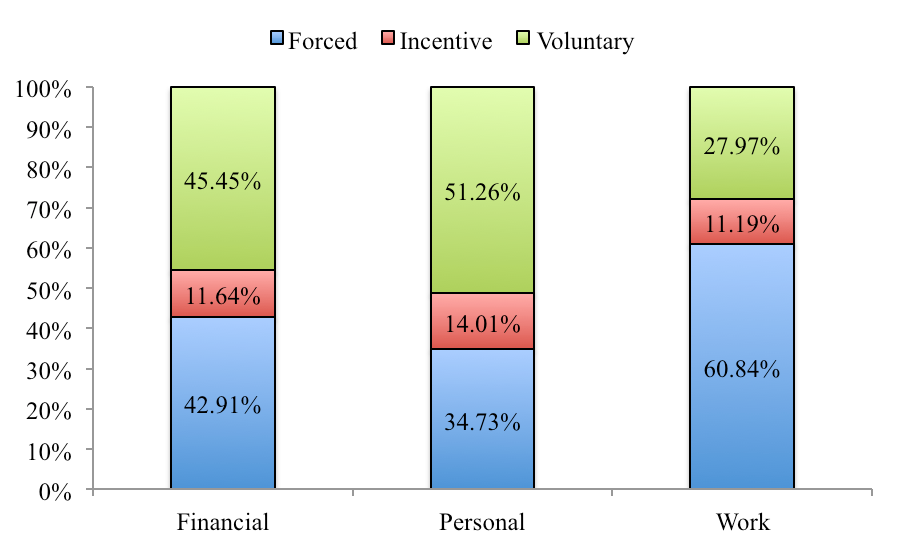
\includegraphics[width=0.95\textwidth]{assets/motivation.png}
  \end{center}
  \caption[Motivation für die Nutzung von \acs{2FA} in verschiedenen Kontexten]{Motivation für die Nutzung von \acs{2FA} in verschiedenen Kontexten.\\\parencite[6]{decristofaroComparativeUsability2014}}
  \label{fig:motivation}
\end{figure}

% \parencite{gargHeuristicsBiases2013} (7 in \textcite{dasWhyJohnny2018})

\textcite{dasWhyJohnny2018} nennen ein mangelndes Bewusstsein für Sicherheitsrisiken und die daraus entstehende Wahrnehmung, dass die Verwendung von \ac{2FA} keinen Mehrwert hat, als primären Grund für die mangelnde Akzeptanz von \ac{2FA}. In der Studie von \textcite{ackermanImpedimentsAdoption2020} wurde ein ähnliche Meinung als zweithäufigster Grund\footnote{Am häufigsten wurde fehlende Zeit als Grund genannt. Abgesehen von Möglichkeiten, den Einrichtungsprozess zu optimieren und darüber zu informieren, soll hier jedoch der Augenmerk auf inhaltlichen Gründen liegen.} genannt, \ac{2FA} nicht einzurichten. Die Teilnehmerinnen glaubten nicht, dass ihre Accounts Ziel von Cyberattacken werden könnten \parencite{ackermanImpedimentsAdoption2020}. Um Nutzerinnen zu überzeugen, \ac{2FA} zu nutzen, hilft es, sie darüber aufzuklären. Dazu ist eine Nachricht, welches Risiken auf einem persönlichen Level aufdeckt, eine Gegenmaßnahme (Nutzung von \ac{2FA}) vorschlägt und zeigt, wie einfach die Umsetzung dieser ist, geeignet \parencite{ackermanImpedimentsAdoption2020}.

Zu beachten ist jedoch, dass laut \textcite{ackermanImpedimentsAdoption2020} eine erhöhte Wahrnehmung des Stärkegrades der Risiken nicht zu einer höheren Einführungsrate von \ac{2FA} führte. Die Nutzerinnen reagieren also nicht in einem verstärkten Maße auf drohende Nachrichten \parencite{ackermanImpedimentsAdoption2020}.

Abgesehen von den Risiken der Nichtnutzung sollten auch die Vorteile der Nutzung von \ac{2FA} kommuniziert werden, da Menschen Entscheidungen treffen, indem sie Vorteile und Risiken miteinander abwägen \parencite{dasWhyJohnny2018}. Dieser Theorie folgend sollten Sicherheitssystem konstruiert werden, um die Verbreitung zu verbessern \parencite{gargHeuristicsBiases2013}.

\pskip
In der Studie von \textcite{dasWhyJohnny2018} wurde mehrfach geäußert, dass die Teilnehmerinnen bereits vollstes Vertrauen in ihre Sicherheitsvorkehrungen und Passwortwahl hatten. Damit einher ging ein Missverständnis über die Funktionsweise von \ac{2FA}, welcher von \textcite{ackermanImpedimentsAdoption2020} als dritthäufigster Grund genannt wurde, \ac{2FA} nicht einzurichten. Klare Kommunikation kann auch Unsicherheiten über den Einrichtungsprozess, die Funktionsweise und die Zuverlässigkeit von \ac{2FA} beseitigen \parencite{ackermanImpedimentsAdoption2020}.

Im gleichen Kontext ist eine Gruppe von Nutzerinnen zu erwähnen, denen Vertrauen in die eigene Fähigkeit, \ac{2FA} einzurichten und zu nutzen, fehlt \parencite{ackermanImpedimentsAdoption2020}. \textcite{ackermanImpedimentsAdoption2020} betont, dass dieses Selbstvertrauen benötigt wird, um Nutzerinnen dazu zu bewegen, \ac{2FA} zu nutzen.

\pskip
\textcite{dasWhyJohnny2018} schlagen vor, die Vorteile der Nutzung von \ac{2FA} für Nutzerinnen zu vergrößern, um so Anreize zur Nutzung von \ac{2FA} zu schaffen. Der erfahrene Wert von \ac{2FA} wird dadurch gesenkt, dass weiterhin das Passwort ausgedacht, gemerkt und eingegeben werden muss \parencite{dasWhyJohnny2018}. Es wird vorgeschlagen, die Authentifizierung zu vereinfachen, wenn \ac{2FA}-Mittel genutzt werden: Es könnte beispielsweise nicht nach dem vollen Passwort gefragt werden, falls \ac{2FA} auf einem bekannten Gerät genutzt wird \parencite{dasWhyJohnny2018}.

\pskip
\textcite{colnagoItsNot2018} stellen die Wichtigkeit einer guten Implementierung von \ac{2FA} hervor. Dabei sollte sowohl auf die Einrichtung, als auch auf die alltägliche Nutzung geachtet werden, um eine Verärgerung von Nutzerinnen zu verhindern \parencite{colnagoItsNot2018}. Eine gute Implementierung achtet darauf, die Nutzerinnen zu unterstützen und weniger negative Situationen zu schaffen \parencite{colnagoItsNot2018}.

In institutionellen Kontexten stellen \ac{2FA}-Pflichten ein valides Mittel dar, um Nutzungsraten zu verbessern. Während bei einer Durchsetzung durch Pflicht mehr negative Erfahrungen aufgezeichnet wurden, sagten die Nutzerinnen auch aus, dass es einfacher als erwartet war, \ac{2FA} zu nutzen \parencite{colnagoItsNot2018}. Vielleicht können solche Erfahrungen auch das Nutzungsverhalten bei privaten Anwendungen beeinflussen.

\chapter{Fazit}

Im Rahmen dieser Arbeit wurden die Sicherheit und die Usability verschiedener \acl{2FA}-Methoden untersucht. Die Ergebnisse verdeutlichen, dass jede der betrachteten Methoden - von \acp{OTP}, \acp{TOTP}, vor-generierten Codes, Push-Benach\-richtigungen bis hin zu \ac{U2F}-Security-Keys - sowohl Vor- als auch Nachteile aufweist.

Obwohl \ac{U2F}-Security-Keys die höchste Sicherheit bieten, werden sie in der Praxis aufgrund ihrer höheren Einrichtungs­komplexität und der Notwendigkeit eines zusätzlichen physischen Geräts weniger genutzt. Im Gegensatz dazu erfreuen sich \acp{OTP} über SMS und E-Mail trotz ihrer Sicherheitsrisiken großer Beliebtheit, da sie bereits bekannt sind und ohne zusätzliche Hardware einfach verwendet werden können.

Die Untersuchung hat zudem gezeigt, dass die Verbreitung von \ac{2FA} im privaten Bereich trotz der bekannten Sicherheitsvorteile weiterhin gering ist. Dies liegt häufig an einer Mischung aus mangelndem Bewusstsein für die Bedrohungen und der Wahrnehmung, dass der zusätzliche Aufwand der Nutzung von \ac{2FA} keinen signifikanten Sicherheitsvorteil bietet. Um die Akzeptanz von \ac{2FA} zu steigern, sollten sowohl die Usability der Verfahren verbessert als auch die Vorteile klarer kommuniziert werden.

Zukünftige Forschung sollte sich darauf konzentrieren, die Usability von \ac{2FA}-Methoden weiter zu optimieren, insbesondere im Hinblick auf die Einstiegshürden bei sicheren Methoden wie \ac{U2F}-Security-Keys. Zudem könnten Anreize und bessere Aufklärungskampagnen dazu beitragen, die Akzeptanz in der breiten Bevölkerung zu fördern. So könnte \ac{2FA} zu einem festen Bestandteil des Alltags vieler Nutzerinnen werden und mehr Accounts effektiv schützen.


%
% Anhang
%

% \begin{appendices}
% \part*{Anhang}
% \end{appendices}


% \nocite{*}
\cleardoublepage
\pdfbookmark[-1]{Literaturverzeichnis}{literature}
\chapter*{Literaturverzeichnis}
\printbibliography[heading=none]

\cleardoublepage
\pdfbookmark[-1]{Selbstständigkeitserklärung}{independence}
\begin{tucerklaerung}
  \vspace{1em}\noindent
  Ich erkläre gegenüber der Technischen Universität Chemnitz, dass ich das vorliegende \type{} selbstständig und ohne Benutzung anderer als der angegebenen Quellen und Hilfsmittel angefertigt habe.

  \vspace{1em}\noindent
  Die vorliegende Arbeit ist frei von Plagiaten. Alle Ausführungen, die wörtlich oder inhaltlich aus anderen Schriften entnommen sind, habe ich als solche kenntlich gemacht.

  \vspace{1em}\noindent
  Diese Arbeit wurde in gleicher oder ähnlicher Form noch bei keinem anderen Prüfer als Prüfungsleistung eingereicht und ist auch noch nicht veröffentlicht.


  \begin{flushright}
    \place, \makeatletter\@date\makeatother
  \end{flushright}
  \vspace{\baselineskip}
  \begin{flushright}
    
\includegraphics[height=2.5\baselineskip]{assets/signature.pdf}\\
    Joshua Jeschek
  \end{flushright}
\end{tucerklaerung}

\end{document}
